\section{Примеры внутреннего "убранства"}\label{part_example_of_doc_inside}
\subsection{Оформление доп. объектов}\label{part_pasting_of_extra_objects}
\subsubsection{Вставка рисунков}\label{part_pasting_of_figures}
Пример оформления рисунка~--- см.~ниже по тексту.

\begin{figure}[h]
	\centering
	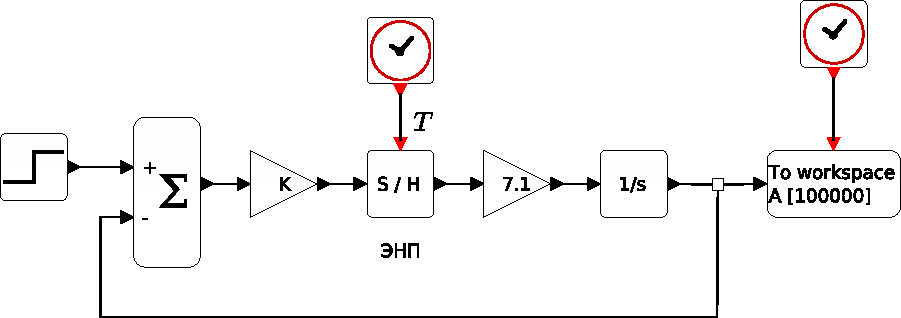
\includegraphics[width=0.7\textwidth]{scheme.pdf}
	\caption{Схема моделирования простенького ОУ.}
	\label{figure_just_example}
\end{figure}


\subsubsection{Вставка таблиц}\label{part_pasting_of_tables}
Пример оформления таблицы~--- см.~ниже по тексту.

\begin{table}[h]
	\caption{Параметры Денавита-Хартенберга.}
	\begin{tabular}{|c|c|c|c|c|}
		\hline
		Звено & $a_i$ & $\alpha_i$ & $d_i$ & $\theta_i$\\
		\hline
		1 & 0 & $\pi/2$ & $l_1$ & $\varphi_1+\pi/2$\\
		\hline
		2  & $l_2$ & $\pi$ & $s_1-2r$ & $\varphi_2-\pi/2$\\
		\hline	
		3 & $l_3$ & $-\pi/2$ & $s_2-2r$ & $-\varphi_3$\\
		\hline
		4 & $l_4$ & $-\pi/2$ & $s_3-2r$ & $-\varphi_4$\\
		\hline
		5 & $l_5$ & $-\pi/2$ & $s_4-2r$ & $-\varphi_5$\\
		\hline
		6 & $l_6$ & $-\pi/2$ & $s_5-2r$ & $-\varphi_6$\\
		\hline
	\end{tabular}
	\label{table_DH_params}
\end{table}


\subsubsection{Вставка формул}\label{part_pasting_of_formulas}
Пример оформления формулы:
\begin{equation}\label{eq_example_of_formula}
	W(s) = \cfrac{T_ms+1}{T_ms^2+T_es+1}
\end{equation}
где $T_m$~--- первая постоянная, а $T_e$~--- вторая.

\subsection{Оформление cсылок}\label{part_editing_of_refs}
Ссылка на раздел~--- \ref{part_example_of_doc_inside}.
Ссылка на подраздел~--- \ref{part_pasting_of_extra_objects}.
Ссылка на что-то меньшее подраздела~--- \ref{part_pasting_of_figures}.
Ссылка на рисунок~--- \ref{figure_just_example}.
Ссылка на таблицу~--- \ref{table_DH_params}.
Ссылка на формулу~--- \eqref{eq_example_of_formula}.
Ссылка на источник~--- \cite{UrcolaIROS08}\footnote{Описание описания источника~--- см.~used\_books.bib.}.
\newpage